\question[10] Miguel tiene bloques de plástico de igual tamaño y arma una torre con todos ellos. Observa la imagen:

\begin{minipage}{0.4\linewidth}
    \begin{figure}[H]
        \centering
        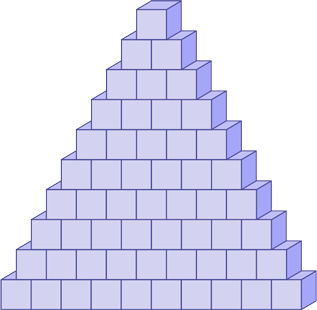
\includegraphics[width=0.7\linewidth]{../images/22bc4d835622314209af99a305ea2515952e3902}
        \caption{Torre con bloques.}
        \label{fig:22bc4d835622314209af99a305ea2515952e3902}
    \end{figure}
\end{minipage}\hfill
\begin{minipage}{0.6\linewidth}
    Si Miguel armara una torre de 32 filas,
    \textbf{¿cuántos bloques necesitará en total?}
    \begin{solutionbox}{1.2cm}
        528 bloques.
    \end{solutionbox}
\end{minipage}
